
\section{Background}
\label{sec:back}
\vspace{-.2cm}
%\subsection{GPU Architecture and Resource Sharing}
Driven by the demand for high-throughput capabilities, the GPU has evolved to leverage massive 
parallelism with a many-core design to provide huge computational throughput and memory bandwidth. 
The cores of NVIDIA GPUs are called Streaming Multiprocessors, each of which can simultaneously 
host multiple active thread blocks (also known as Cooperative Thread Array) contexts. 
The number of active thread blocks that an SM can host depends on the hardware resource of the SM 
(i.e., register file size) and the resource requirement of the thread blocks. 
When a thread block runs on an SM, it is executed in a SIMD fashion with 32 threads (called a warp) at a time. 
	\begin{figure}
\vspace{-.25in}
		\centering
		\begin{minipage}{0.45\linewidth}
		%\centering
		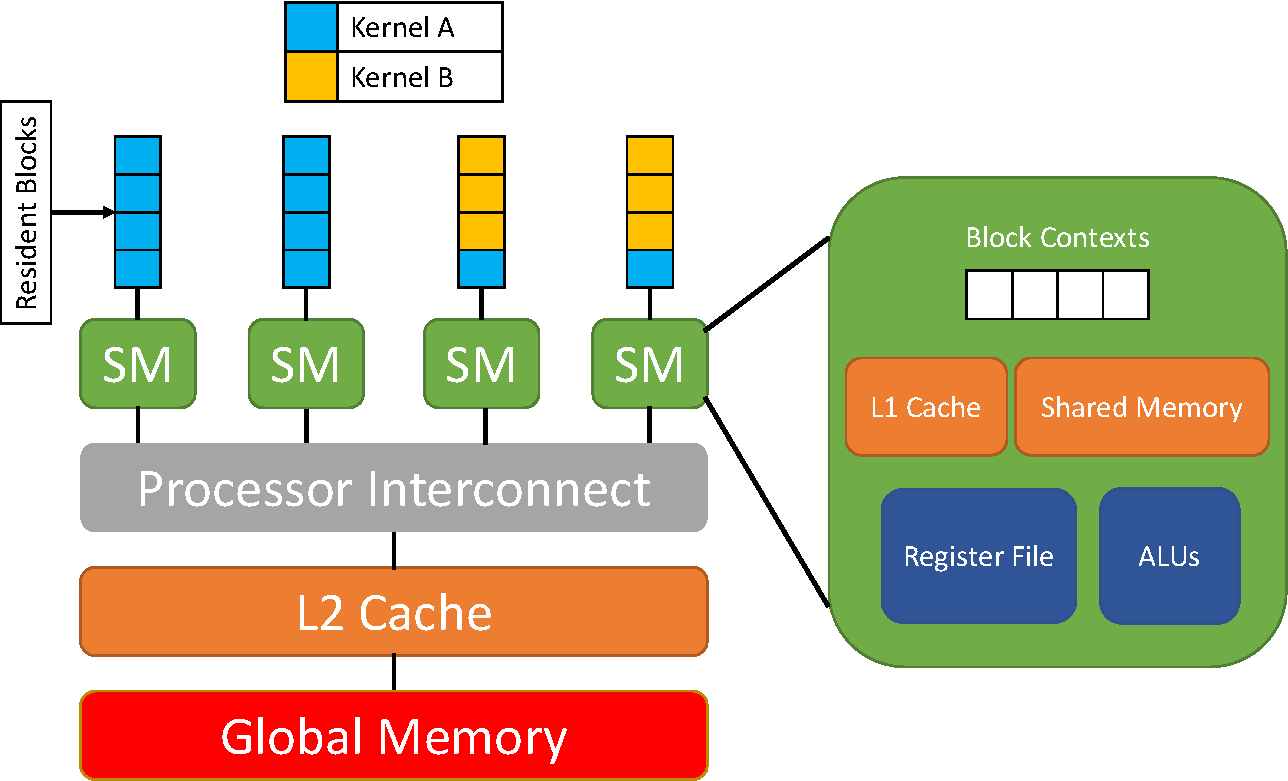
\includegraphics[width=\linewidth]{figures/gpu_diagram_cropped.pdf}
		\caption{Graphics Processing Unit (GPU)}
		\label{fig:gpu}
		\end{minipage}
	%    subfloat[fig:gpu]
		\hfill
		\begin{minipage}{0.45\linewidth}
		%\centering
		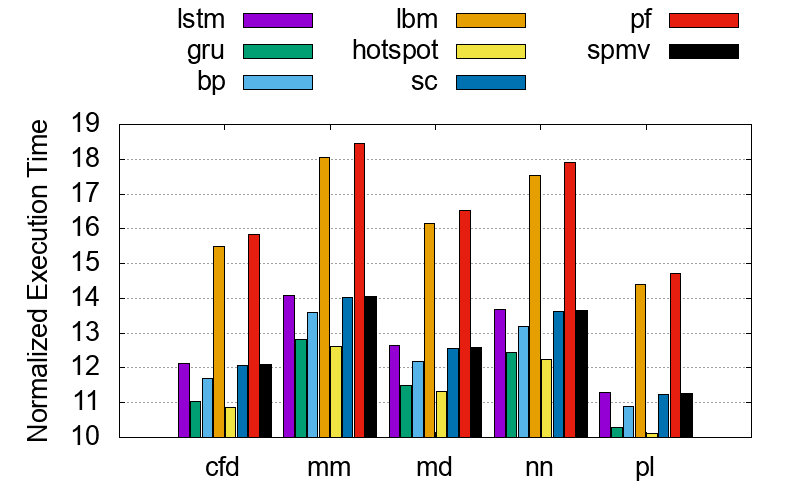
\includegraphics[width=\linewidth]{figures/seq_time.png}
		\caption{QoS violation for co-runs when the GPU is unpreemptable.}
		\label{fig:qos}
		%\vspace{-0.5cm}
		\end{minipage}
		\vspace{-0.6cm}
	\end{figure}

Conceptually, all the thread blocks of the launched kernels wait in a queue.  The hardware implements a FIFO thread block scheduler, which dispatches the waiting thread blocks to SMs as long as the available hardware resource can satisfy the resource demands. Hence, a kernel's thread blocks are guaranteed to be scheduled first before any other thread block of a later launched kernel.

Starting from the Fermi architecture, NVIDIA GPUs support concurrent kernel execution.  Later, NVIDIA introduced the Multi-Process Service (MPS), which enables kernels from  different applications to be executed simultaneously on the same GPU. However, due to significant context switch overhead,  the GPU hardware does not support temporal core sharing.  Consequently, the co-running kernels spatially share a GPU only  when the earlier launched kernel cannot consume all the computational resources. %This situation happens in the following two cases.  First, the earlier launched kernel only subscribes a small number of thread blocks. Second, the earlier launched kernel is about to finish its execution. As seen in Figure 1, the overall resource requirement of kernel A's remaining thread blocks  is so small that the greedy scheduler dispatches kernel B's thread blocks on the device such that kernel B's thread blocks will co-run with those of   kernel A on the last two SMs. 
Due to the organization of the hardware, Fig.~\ref{fig:gpu}  shows an interesting resource sharing scenario. The co-running thread blocks  from both kernel A and B on the same SM compete to use the L1 cache and ALUs and all the currently running thread blocks contend for use of the interconnect, L2 cache and global memory bandwidth.
%\subsection{QoS Issues in Co-Located GPU Applications}
%Most cloud service platforms nowadays employ GPUs \nadd{because of their high throughput and low cost}. But as pointed out by Chen  et al.~\cite{Chen+:ASPLOS16}, the GPUs may experience very low utilization  due to the diurnal pattern and the dynamic behaviors of GPU applications.  A natural solution similar to what exists in CPU-based platforms is \nsout{to co-locate  applications to share the same GPU}{multitasking where multiapplications share the hardware resources}. \nadd{There are two alternatives for multitasking on GPUs, spatial and temporal sharing.} While the co-location indeed improves \nadd{hardware} utilization,  uncoordinated co-running \nadd{applications may} introduce\nsout{s}{} severe performance interference \nadd{to others}and  \nadd{such interference will leads to} violat\nsout{es}{ion} \nadd{of} the QoS requirement of user-facing applications. 
%Baymax models the interference on data transfer between the CPU and the GPU  and the contention on GPU computational resources~\cite{Chen+:ASPLOS16}.  Based on a runtime system, it carefully manages data transfers and reschedules  kernel executions to mitigate the QoS violation issue. However, Baymax assumes  the GPU cannot be preempted, so once a kernel is launched,  it may monopolize the whole GPU for a long time, leading to unacceptable  performance degradation for the waiting kernels. In this paper, we  focus on the complicated problem of GPU core sharing between co-running  GPU applications and assume that the contention on data transfer is handled by the model proposed in Baymax.
